\chapter{Non-Uniform Encoding and Applications}\chlabel{nuel}
The partial prefix-free codes designed and studied in this chapter
will all be denoted $C : \Omega \to \{0, 1\}^* \cup \{\bot\}$, where
$\Omega$ is to be understood from context.

\section{The Non-Uniform Encoding Lemma}

We can extend \lemref{uel} to handle non-uniform input distributions
with a result of Barron, and independently rediscovered through a
joint effort between Devroye, Lugosi, and
Morin~\cite{devroye:workshop}. First, recall the following classic
result.

\begin{thm}[Markov's Inequality]\thmlabel{markov}
  For a non-negative random variable $X$ with finite expectation, and
  any $a > 0$,
  \[
  \Pr[X \geq a] \leq \E[X]/a .
  \]
\end{thm}

\begin{lem}[Barron~\cite{barron:dissertation}]\lemlabel{nuel}
  Let $C : \Omega \to \{0, 1\}^* \cup \{\bot\}$ be a partial
  prefix-free code. Let $x \in \Omega$ be chosen with probability
  $p_x$. Then, for any $s \geq 0$,
  \[\Pr\left[\,|C(x)| \leq \log (1/p_x) - s\,\right]
  \leq 2^{-s}.\]
\end{lem}
\begin{proof}
  We see that
  \begin{align}
    \Pr\left[\,|C(x)| \leq \log(1/p_x) - s\,\right] & = \Pr\left[\,\log(1/p_x) - |C(x)| \geq s\,\right] \notag \\
    & = \Pr\left[2^{\log(1/p_x) - |C(x)|} \geq 2^s\right] \notag \\
    & \leq 2^{-s} \E\left[2^{\log(1/p_x) - |C(x)|}\right] \eqlabel{non-uniform-part}
  \end{align}
  by Markov's inequality. Further, by definition of the expected
  value, \eqref{non-uniform-part} becomes
  \begin{align*}
    2^{-s} \E\left[\,2^{\log(1/p_x) - |C(x)|}\,\right] = 2^{-s} \left(\sum_{C(x) \neq \bot} p_x 2^{\log(1/p_x) - |C(x)|}\right) = 2^{-s} \left(\sum_{C(x) \neq \bot} 2^{-|C(x)|} \right).
  \end{align*}
  By \lemref{kraft-inequality},
  $\sum_{C(x) \neq \bot} 2^{-|C(x)|} \leq 1$, and the result is
  obtained.
\end{proof}

Indeed, this non-uniform encoding lemma immediately implies
\lemref{uel} by choosing $p_x = 1/|\Omega|$.

\begin{prop}\proplabel{non-uniform-binary-runs-loose}
  Let $x_1, \ldots, x_n$ be independent $\text{Bernoulli}(p)$ random
  variables. Then, the probability that $x = x_1 \cdots x_n \in \{0,
  1\}^n$ has a run of ones of length at least
  \[\frac{s + \ceil{\log n} + 1}{\log (1/p)}\]
  is at most $2^{-s}$.
\end{prop}
\begin{proof}
  The proof is almost identical to that of
  \propref{binary-runs}. Suppose that $x$ has a run of ones of length
  $t \geq (s + \ceil{\log n} + 1)/\log (1/p)$.

  Our code begins with the index where this run begins, which allows
  us to deduce $t$ one bits of $x$; and then the Shannon-Fano code
  with parameter $p$ for the remaining bits. Recall that $n_1(x)$ and
  $n_0(x)$ denote the number of one and zero bits in $x$,
  respectively. In total, this code has length
  \begin{align*}
    |C(x)| &= \ceil{\log n} + \left\lceil (n_1(x) - t) \log \frac{1}{p} + n_0(x) \log \frac{1}{1 - p} \right\rceil \\
           &\leq \log \frac{1}{p_x} + \ceil{\log n} - t \log \frac{1}{p} + 1 \\
           &\leq \log \frac{1}{p_x} - s
  \end{align*}
  by our choice of $t$, and since $p_x = p^{n_1(x)} (1 -
  p)^{n_0(x)}$. The result follows from \lemref{nuel}.
\end{proof}

This result appears even more unnatural than that of
\propref{binary-runs}---again, we can prove that this bit string has a
run of length at least $(s + \log n)/\log (1/p)$ by appealing directly
to probability. We will show how this can be resolved in \chref{el}.

\section{The Erd\H{o}s-R\'{e}nyi Random Graph}

\begin{defn}
  The \emph{Erd\H{o}s-R\'{e}nyi random graph} $G_{n, p}$ is the space
  of random undirected graphs on $n$ vertices in which each edge is
  included independently at random with probability $p$.
\end{defn}

The study of the Erd\H{o}s-R\'{e}nyi random graph model played an
important role in the popularization of the now pervasive
probabilistic method~\cite{alon:probabilistic, erdos:randomgraphs}. In
general, probabilistic proofs appear to be easily adapted into
encoding arguments. We show how it is simple to recover some of
Erd\H{o}s and R\'{e}nyi's classic results about $G_{n, p}$.

\begin{lem}\lemlabel{erdos-renyi-lemma}
  The probability that $G \in G_{n, p}$ has a partition $(U, W)$ of
  its vertex set such that $|U| = k$ and there is no edge of $G$ with
  one endpoint in $U$ and the other in $W$ is at most
  $O\left({n \choose k} (1 - p)^{k (n - k)}\right)$.
\end{lem}
\begin{proof}
  We encode $G$ by giving its adjacency matrix $A$, which determines
  the graph. The entire matrix is determined by its portion which lies
  above its diagonal, which is a random bit string of length
  $\binom{n}{2}$ in which each bit appears with probability $p$.

  We give a list of the $k$ vertices in $U$, which determines
  $k(n - k)$ non-edges of the graph between $U$ and $W$; and a
  Shannon-Fano code with parameter $p$ for the remaining
  $\binom{n}{2} - k(n - k)$ edges of the graph. This code has length
  \begin{align*}
    |C(G)| &\leq \log {n \choose k} + n_1(A) \log \frac{1}{p} + (n_0(A) - k(n - k)) \log \frac{1}{1 - p} + O(1) \\
           &= \log \frac{1}{p_G} + \log {n \choose k} - k(n - k) \log \frac{1}{1 - p} + O(1) \\
           &= \log \frac{1}{p_G} + \log \left(O\left({n \choose k} (1 - p)^{k(n - k)}\right)\right).
  \end{align*}
  We finish by applying \lemref{nuel}.
\end{proof}

The typical proof of the above result, given by the probabilistic
method, says that this probability is at most
$\binom{n}{k} (1 - p)^{k (n - k)}$. Nevertheless,
\lemref{erdos-renyi-lemma} is sufficient to obtain the classic
threshold connectivity results for the Erd\H{o}s-R\'{e}nyi random
graph.

%As a first application of \lemref{erdos-renyi-lemma}, we establish
%connectivity properties of $G_{n, p}$:
%
\begin{thm}
  When $p = (1 + \eps) \frac{\ln n}{n}$, $G \in G_{n, p}$ has no
  isolated vertices with high probability.
\end{thm}
\begin{proof}
  Choose $k = 1$ in \lemref{erdos-renyi-lemma}. Then, the probability
  that $G$ has an isolated vertex is at most
  \[
  O\left(n \left(1 - (1 + \eps) \frac{\ln n}{n}\right)^{n - 1}\right) =  O\left(n e^{-(1 + \eps) \ln n} (1 + o(1))\right) = O(n^{-\eps}). \hfill \qedhere
  \]
\end{proof}
%We can apply \lemref{erdos-renyi-lemma} and the union bound to show
%that $G$ is connected with high probability.

\begin{thm}
  When $p = (1 + \eps) \frac{\ln n}{n}$, $G \in G_{n, p}$ is
  connected with high probability.
\end{thm}
\begin{proof}
  This follows from \lemref{erdos-renyi-lemma} and the union bound.
\end{proof}
%\begin{proof}
%  By the union bound, the probability that $G$ is disconnected is at
%  most:
%  \begin{align*}
%    \sum_{k = 1}^{n/2} O({n \choose k} (1 - p)^{k(n - k)}) & \leq O(1)\sum_{k = 1}^n {n \choose k} ((1 - p)^{n/2})^k \\
%    & = O(1)[((1 - p)^{n/2} + 1)^n - 1]
%  \end{align*}
%
%  Moreover, since $1 + x \leq e^x$ for all $x \in \R$, we see that
%  \begin{align*}
%    ((1 - p)^{n/2} + 1)^n - 1 & \leq (e^{-pn/2} + 1)^n - 1 \leq e^{e^{-pn^2/2}} - 1 \\
%                              & \leq e^{n^{-(1 + \eps)n/2}} - 1 \to 0
%  \end{align*}

 % $(1 - 1/n)^n = e^{-1} + O(1/n)$

 % $(1 - 1/(n/\ln n^{1+\eps}))^{n} = (e^{-1} + O(\ln n/n))^{\ln n^{1+\eps}}$

 % $= n^{-(1 + \eps)/2} + O(\ln^2 n/n^{2 + \eps})$
  
  %Since $\left(1 - \frac{1}{n}\right)^n = e^{-1} + O(1/n)$, we see
  %that:
  %\begin{align*}
  %  (1 - p)^{n/2} & = \left(1 - (1 + \eps) \frac{\ln n}{n}\right)^{n/2} = n^{-(1 + \eps)/2} + O\left(\frac{\log^2 n}{n^{(3 + \eps)/2}}\right)
  %\end{align*}

  %If $\lim (1 + f(n)) = 1$, then $\lim (1 + f(n))^n = 1$.

  %$\lim e^{n \ln (1 + f(n))}$

  %It can be shown that this probability tends to $0$.
%\end{proof}

%\begin{thm}
%  When $p = (1 - \eps) \frac{\ln n}{n}$, $G \sim G_{n, p}$ is
%  disconnected with high probability.
%\end{thm}
%\begin{proof}
%  Again, we encode $G$'s adjacency matrix $A$.
%
%  If $G$ is connected, then it has a spanning tree $T$. We encode $G$
%  by providing the shape of $T$, fixing an arbitrary vertex as its
%  root, which informs us of the presence of $n - 1$ edges in $G$; and
%  then a Shannon-Fano code for the remaining edges in the graph. This
%  costs:
%  \begin{align*}
%    b & \leq (n - 2)\log n + (n_1(A) - (n - 1)) \log \frac{1}{p} + n_0(A) \log \frac{1}{1 - p} + 1 \\
%      & = \log \frac{1}{p_A} + (n - 2) \log n + (n - 1) \log p \\
%      & = \log \frac{1}{p_A} - \log n + (n - 1)\log \ln n^{1 - \eps}
%  \end{align*}%

%  bits. By \lemref{nuel}, we obtain that $G$ is connected with
%  probability $O(\ln n/n)$, so $G$ is disconnected with high
%  probability.
%\end{proof}

\begin{thm}\thmlabel{erdos-renyi-component}
  When $p = \frac{1}{\alpha n}$ for $\alpha > e$, the graph
  $G \in G_{n, p}$ has a component of size at least
  \[
  \frac{\log n + s + O(1)}{\log (\alpha/e)}
  \]
  with probability at most $2^{-s}$.
\end{thm}
\begin{proof}
  We again encode the adjacency matrix $A$ of $G$. Suppose that $G$
  has a component of size $t$. We encode $G$ by giving these $t$
  vertices; the shape of a spanning tree for this component; and a
  Shannon-Fano code with parameter $p$ for the remaining edges of the
  graph. This code has length
  \begin{align*}
    |C(G)| &\leq \log \binom{n}{t} + (t - 2) \log t + (n_1(A) - (t - 1))\log \frac{1}{p} + n_0(A) \log \frac{1}{1 - p} + O(1) \\
           &\leq \log \frac{1}{p_G} + t \log n - t \log t + t \log e + t \log t - (t - 1) \log \frac{1}{p} + O(1) \tag{by \eqref{binom-code-loose}} \\
           &\leq \log \frac{1}{p_G} + \log n + t \log e - t \log \alpha + O(1) \\
           &= \log \frac{1}{p_G} + \log n - t \log \frac{\alpha}{e} + O(1) \\
           &\leq \log \frac{1}{p_G} - s
  \end{align*}
  by our choice of $t$. We finish by applying \lemref{nuel}.
\end{proof}
\begin{rem}
  This result and its proof are similar to that of
  \lemref{two-choice-component-size} from our study of random
  multigraphs in 2-choice hashing. Indeed, the random multigraph we
  studied contained exactly $n$ edges for $cn$ vertices,
  \emph{i.e.}~$n/c$ edges for $n$ vertices, and the
  Erd\H{o}s-R\'{e}nyi graph from \thmref{erdos-renyi-component} is
  expected to contain $(n - 1)/(2 \alpha)$ edges for $n$
  vertices. Since the random graph models are so similar, and since
  the edge densities we are concerned with are practically identical,
  this observation should be of no surprise.
\end{rem}

A triangle in a graph is a $K_3$ subgraph. Our nextt encoding argument
bounds the probability that $G_{n, c/n}$ has no triangle. It is easy
to see that the expected number of triangles in $G_{n, c/n}$ is
$\binom{n}{3} (c/n)^3 = c/6 - O(1/n)$, so $G_{c, c/n}$ is expected to
have at least one triangle for large enough values of $c$. However, a
typical proof that $G_{n, c/n}$ has a triangle with non-negligible
probability usually uses the second moment method which involves
computing the variance of the number of
triangles~\cite{souza:notes}. To show that $G_{n, c/n}$ has a triangle
with exponential probability is even more complicated, and a proof of
this result would still typically rely on an advanced probabilistic
inequality~\cite{alon:probabilistic}. Our argument is easy and avoids
this trouble.

We will, however, rely on the following classic result, which we later
prove in \chref{el} using an encoding argument.
\newtheorem*{thm:chernoff}{Theorem 5.7}%{\begin{NoHyper}\thmref{chernoff}\end{NoHyper}}
%\newreptheorem{theorem}{Theorem}
\begin{thm:chernoff}[Additive Chernoff Bound~\cite{mulzer:encoding}]
  Let $B$ be a $\text{Binomial}(n, p)$ random variable. Then
  \[
  \Pr[B \leq (p - t)n] \leq 2^{-n D(p - t \| p)}
  \]
  where
  \[D(p \| q) = p \log \frac{p}{q} + (1 - p) \log \frac{1 - p}{1 -
    q}\]
  is the \emph{Kullback-Leibler divergence} or \emph{relative entropy}
  between Bernoulli random variables with parameters $p$ and $q$.
\end{thm:chernoff}

\begin{figure}
  \centering
  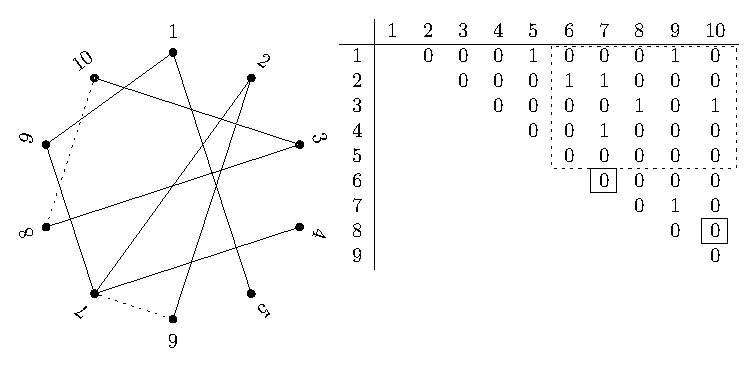
\includegraphics{triangles}
  \caption{The random graph $G_{n, c/n}$ has triangles when $c$ is
    large enough. The depicted zero bits in the adjacency matrix can
    be deduced from the first $n/2$ rows.}
  \figlabel{triangles}
\end{figure}

\begin{thm}\thmlabel{triangles-up}
  When $p = c/n$, the graph $G \in G_{n, p}$ contains at least one
  triangle with probability at least $1 - 2^{-\varOmega(c^3)}$.
\end{thm}
\begin{proof}
  Refer to \figref{triangles}. Suppose that $G$ contains no
  triangles. We encode the adjacency matrix $A$ of $G$. Let $M$ be the
  $n/2 \times n/2$ submatrix of $A$ determined by the rows
  $1, \ldots, n/2$ and the columns $n/2 + 1, \ldots, n$. Note that
  $\E[n_1(M)] = cn/4$.

  Suppose that $n_1(M) < cn/8$. Note that $n_1(M)$ is a
  $\text{Binomial}(n^2/4, c/n)$ random variable whose value deviates
  largely from its mean. Then, by Chernoff's bound, we obtain that
  \begin{align*}
    \Pr[n_1(M) < cn/8] &= \Pr[n_1(M) < (c/2n) (n^2/4)] \leq 2^{-(n^2/4) D(c/2n \| c/n)}.
  \end{align*}
  The function $D(x/2 \| x) : [0, 1] \to \R$ has
  derivative
  \[\frac{d}{dx} D(x/2 \| x) = - \frac{1}{2} + \log \frac{1 - x}{1 -
    x/2} + \frac{\log e}{2(1 - x)}\]
  which is strictly increasing, so
  $D(x/2 \| x) \geq \left(\frac{\log e - 1}{2}\right)x$. Thus,
  $D(c/2n \| c/n) = \varOmega(c/n)$, and
  \[\Pr[n_1(M) < cn/8] \leq 2^{-\varOmega(cn)}.\]

  Suppose instead that $n_1(M) \geq cn/8$. Note that if $A_{i,j} = 1$
  and $A_{i, k} = 1$ for $i < j < k$, then $A_{j, k} = 0$ since $G$
  has no triangles. Let $m_i$ denote the number of ones in the
  $i$\textsuperscript{th} row of $M$. Since the function $x(x - 1)/2$
  is convex, then by \thmref{jensen}, we have that
  \[
  \frac{1}{n/2} \sum_{i = 1}^{n/2} {m_i \choose 2} \geq \binom{2
    n_1(M)/n}{2}.
  \]
  From these observations, we see that by specifying the rows $1,
  \ldots, n/2$ of $A$, we can deduce
  \[m = \sum_{i = 1}^{n/2} {m_i \choose 2} \geq \frac{n}{2} {2 n_1(M)/n
    \choose 2} \geq \frac{n}{2} {c/4 \choose 2} = \varOmega(c^2 n)\]
  zero bits in the rows $n/2 + 1, \ldots, n$.

  We encode $G$ by giving a Shannon-Fano code with parameter $p$ for
  the first $n/2$ rows of $A$; and a Shannon-Fano code with parameter
  $p$ for the rest of $A$, excluding the bits which can be deduced
  from the preceding information. Such a code has length
  \begin{align*}
    |C(G)| &\leq n_1(A) \log \frac{1}{p} + (n_0(A) - m) \log \frac{1}{1 - p} + O(1) \\
           &= \log \frac{1}{p_G} - m \log \frac{1}{1 - p} + O(1) \\
           &\leq \log \frac{1}{p_G} - mp + O(1) \\
           &\leq \log \frac{1}{p_G} - \varOmega(c^3).
  \end{align*}
  Applying \lemref{nuel}, we see that $G$ has no triangles with
  probability at most $2^{- \varOmega(c^3)}$.
\end{proof}

\begin{thm}\thmlabel{triangles-down}
  When $p = \frac{1}{\alpha n}$, $G \in G_{n, p}$ has no triangle
  with probability $1 - O(\alpha^{-3})$.
\end{thm}
\begin{proof}
  Suppose that $G$ contains a triangle. We encode the adjacency matrix
  $A$ of $G$. First, we specify the triangle's vertices; and finish
  with a Shannon-Fano code with parameter $p$ for the remaining
  vertices of the graph. This code has length
  \begin{align*}
    |C(G)| &\leq 3 \log n + (n_1(A) - 3) \log \frac{1}{p} + n_0(A) \log \frac{1}{1 - p} + O(1) \\
           &= \log \frac{1}{p_G} + 3 \log n - 3 \log \frac{1}{p} + O(1) \\
           &= \log \frac{1}{p_G} - 3 \log \alpha + O(1) \\
           &= \log \frac{1}{p_G} - \log O(\alpha^3).
  \end{align*}
  We finish by applying \lemref{nuel}.
\end{proof}

Together, \thmref{triangles-up} and \thmref{triangles-down} establish
that $1/n$ is a threshold function for triangle-freeness.

\section{Percolation on the Torus}

Percolation theory studies the emergence of large components in random
graphs. We give an encoding argument proving that percolation occurs
on the torus when edge survival rate is greater than $2/3$. Our line
of reasoning follows what is known as a \emph{Peierls argument}. For
more precise results, including a general study of percolation theory,
see the book by Grimmett~\cite{grimmett:percolation}.

\begin{defn}
  When $\sqrt{n}$ is an integer, the \emph{$\sqrt{n} \times \sqrt{n}$
    torus grid graph} is defined to be the graph with vertex set
  $\{1, \ldots, \sqrt{n}\}^2$, where $(i, j)$ is adjacent to
  $(k, \ell)$ if
  \begin{itemize}
    \item $|i - k| \equiv 1 \pmod{\sqrt{n}}$ and $|j - \ell| = 0$, or
    \item $|i - k| = 0$ and $|j - \ell| \equiv 1 \pmod{\sqrt{n}}$.
    \end{itemize}
\end{defn}

\begin{thm}
  Let $G$ be the subgraph of the $\sqrt{n} \times \sqrt{n}$ torus grid
  graph in which each edge is chosen with probability $p < 1/3$. Then,
  the probability that $G$ contains a cycle of length at least
  \[\frac{s + \log n + O(1)}{\log (1/(3p))}\]
  is at most $2^{-s}$.
\end{thm}
\begin{proof}
  Let $A$ be the bitstring of length $2n$ encoding the existence of
  edges in $G$. Suppose that $G$ contains a cycle $C'$ of length
  $t \geq (s + \log n + O(1))/\log (1/(3p))$. Encode $A$ by giving a
  single vertex $u$ in $C'$; the sequence of directions that the cycle
  moves along from $u$; and a Shannon-Fano code with parameter $p$ for
  the remaining edges of $G$.

  Note that there are four possibilities for the direction of the
  first step taken by $C'$ from $u$, but only three for each
  subsequent choice. Thus, this sequence can be specified by
  $\lceil 2 + (t - 1) \log 3 \rceil$ bits. The total length of our
  code is then
  \begin{align*}
    |C(G)| &\leq \log n + t \log 3 + (n_1(A) - t) \log \frac{1}{p} +
             n_0(A) \log \frac{1}{1 - p} + O(1) \\
           &= \log \frac{1}{p_G} + \log n - t \log \frac{1}{3p} + O(1) \\
           &\leq \log \frac{1}{p_G} - s
  \end{align*}
  by our choice of $t$. We finish by applying \lemref{nuel}.
\end{proof}

The torus grid graph can be drawn in the obvious way without crossings
on the surface of a torus. This graph drawing gives rise to a dual
graph, in which each vertex corresponds to a face in the primal
drawing, and two vertices are adjacent if and only their primal faces
are incident to the same edge. In this sense, the torus grid graph is
self-dual.

The obvious drawing of the torus grid graph also induces drawings for
any of its subgraphs. Such a subgraph also has a dual, where each
vertex corresponds to a face in the dual torus grid graph, and two
vertices are adjacent if and only if their corresponding faces are
incident to the same edge of the original subgraph.

\begin{thm}
  Let $G$ denote the subgraph of the $\sqrt{n} \times \sqrt{n}$ torus
  grid graph in which each edge is chosen with probability greater
  than $2/3$. Then, $G$ has at most one component of size
  $\omega(\log^2 n)$ with high probability.
\end{thm}
\begin{proof}
  See \figref{peierls} for a visualization of this phenomenon. Suppose
  that $G$ has at least two components of size $\omega(\log^2
  n)$. Then, there is a cycle of faces separating these components
  whose length is $\omega(\log n)$. From the discussion above, such a
  cycle corresponds to a cycle of $\omega(\log n)$ missing edges in
  the dual graph, as in \figref{peierlsrare}. From the previous
  result, we know that this does not happen with high probability.
\end{proof}

\begin{figure}
  \centering
  \begin{subfigure}[t]{0.4\textwidth}
    \includegraphics{torusrare}
    \caption{When $p = 0.33 < 1/3$, long cycles are rare. Dotted lines show
      missing edges in the dual.}
    \figlabel{peierlsrare}
  \end{subfigure}
  \quad\quad
  \begin{subfigure}[t]{0.4\textwidth}
    \includegraphics{torusdense}
    \caption{When $p = 0.67 > 2/3$, there is likely only one large
      component.}
  \end{subfigure}
  \caption{Random subgraphs of the $20 \times 20$ torus grid graph.}
  \figlabel{peierls}
\end{figure}

%
%\subsection{Random Independent Sets on the Hypercube}
%
%Consider the hypercube $Q_d$ with bipartition $(E, O)$. Let $I$ be a
%uniformly random independent set of $Q_d$. Consider the value
%$t = \max\{|I \cap E|, |I \cap O|\}$.
%
%Suppose that $|I_0| \geq 2^d/5$. Then


%\section{SOMETHING ELSE???}
